% Options for packages loaded elsewhere
\PassOptionsToPackage{unicode}{hyperref}
\PassOptionsToPackage{hyphens}{url}
%
\documentclass[
]{article}
\usepackage{amsmath,amssymb}
\usepackage{iftex}
\ifPDFTeX
  \usepackage[T1]{fontenc}
  \usepackage[utf8]{inputenc}
  \usepackage{textcomp} % provide euro and other symbols
\else % if luatex or xetex
  \usepackage{unicode-math} % this also loads fontspec
  \defaultfontfeatures{Scale=MatchLowercase}
  \defaultfontfeatures[\rmfamily]{Ligatures=TeX,Scale=1}
\fi
\usepackage{lmodern}
\ifPDFTeX\else
  % xetex/luatex font selection
\fi
% Use upquote if available, for straight quotes in verbatim environments
\IfFileExists{upquote.sty}{\usepackage{upquote}}{}
\IfFileExists{microtype.sty}{% use microtype if available
  \usepackage[]{microtype}
  \UseMicrotypeSet[protrusion]{basicmath} % disable protrusion for tt fonts
}{}
\makeatletter
\@ifundefined{KOMAClassName}{% if non-KOMA class
  \IfFileExists{parskip.sty}{%
    \usepackage{parskip}
  }{% else
    \setlength{\parindent}{0pt}
    \setlength{\parskip}{6pt plus 2pt minus 1pt}}
}{% if KOMA class
  \KOMAoptions{parskip=half}}
\makeatother
\usepackage{xcolor}
\usepackage[margin=1in]{geometry}
\usepackage{color}
\usepackage{fancyvrb}
\newcommand{\VerbBar}{|}
\newcommand{\VERB}{\Verb[commandchars=\\\{\}]}
\DefineVerbatimEnvironment{Highlighting}{Verbatim}{commandchars=\\\{\}}
% Add ',fontsize=\small' for more characters per line
\usepackage{framed}
\definecolor{shadecolor}{RGB}{248,248,248}
\newenvironment{Shaded}{\begin{snugshade}}{\end{snugshade}}
\newcommand{\AlertTok}[1]{\textcolor[rgb]{0.94,0.16,0.16}{#1}}
\newcommand{\AnnotationTok}[1]{\textcolor[rgb]{0.56,0.35,0.01}{\textbf{\textit{#1}}}}
\newcommand{\AttributeTok}[1]{\textcolor[rgb]{0.13,0.29,0.53}{#1}}
\newcommand{\BaseNTok}[1]{\textcolor[rgb]{0.00,0.00,0.81}{#1}}
\newcommand{\BuiltInTok}[1]{#1}
\newcommand{\CharTok}[1]{\textcolor[rgb]{0.31,0.60,0.02}{#1}}
\newcommand{\CommentTok}[1]{\textcolor[rgb]{0.56,0.35,0.01}{\textit{#1}}}
\newcommand{\CommentVarTok}[1]{\textcolor[rgb]{0.56,0.35,0.01}{\textbf{\textit{#1}}}}
\newcommand{\ConstantTok}[1]{\textcolor[rgb]{0.56,0.35,0.01}{#1}}
\newcommand{\ControlFlowTok}[1]{\textcolor[rgb]{0.13,0.29,0.53}{\textbf{#1}}}
\newcommand{\DataTypeTok}[1]{\textcolor[rgb]{0.13,0.29,0.53}{#1}}
\newcommand{\DecValTok}[1]{\textcolor[rgb]{0.00,0.00,0.81}{#1}}
\newcommand{\DocumentationTok}[1]{\textcolor[rgb]{0.56,0.35,0.01}{\textbf{\textit{#1}}}}
\newcommand{\ErrorTok}[1]{\textcolor[rgb]{0.64,0.00,0.00}{\textbf{#1}}}
\newcommand{\ExtensionTok}[1]{#1}
\newcommand{\FloatTok}[1]{\textcolor[rgb]{0.00,0.00,0.81}{#1}}
\newcommand{\FunctionTok}[1]{\textcolor[rgb]{0.13,0.29,0.53}{\textbf{#1}}}
\newcommand{\ImportTok}[1]{#1}
\newcommand{\InformationTok}[1]{\textcolor[rgb]{0.56,0.35,0.01}{\textbf{\textit{#1}}}}
\newcommand{\KeywordTok}[1]{\textcolor[rgb]{0.13,0.29,0.53}{\textbf{#1}}}
\newcommand{\NormalTok}[1]{#1}
\newcommand{\OperatorTok}[1]{\textcolor[rgb]{0.81,0.36,0.00}{\textbf{#1}}}
\newcommand{\OtherTok}[1]{\textcolor[rgb]{0.56,0.35,0.01}{#1}}
\newcommand{\PreprocessorTok}[1]{\textcolor[rgb]{0.56,0.35,0.01}{\textit{#1}}}
\newcommand{\RegionMarkerTok}[1]{#1}
\newcommand{\SpecialCharTok}[1]{\textcolor[rgb]{0.81,0.36,0.00}{\textbf{#1}}}
\newcommand{\SpecialStringTok}[1]{\textcolor[rgb]{0.31,0.60,0.02}{#1}}
\newcommand{\StringTok}[1]{\textcolor[rgb]{0.31,0.60,0.02}{#1}}
\newcommand{\VariableTok}[1]{\textcolor[rgb]{0.00,0.00,0.00}{#1}}
\newcommand{\VerbatimStringTok}[1]{\textcolor[rgb]{0.31,0.60,0.02}{#1}}
\newcommand{\WarningTok}[1]{\textcolor[rgb]{0.56,0.35,0.01}{\textbf{\textit{#1}}}}
\usepackage{graphicx}
\makeatletter
\def\maxwidth{\ifdim\Gin@nat@width>\linewidth\linewidth\else\Gin@nat@width\fi}
\def\maxheight{\ifdim\Gin@nat@height>\textheight\textheight\else\Gin@nat@height\fi}
\makeatother
% Scale images if necessary, so that they will not overflow the page
% margins by default, and it is still possible to overwrite the defaults
% using explicit options in \includegraphics[width, height, ...]{}
\setkeys{Gin}{width=\maxwidth,height=\maxheight,keepaspectratio}
% Set default figure placement to htbp
\makeatletter
\def\fps@figure{htbp}
\makeatother
\setlength{\emergencystretch}{3em} % prevent overfull lines
\providecommand{\tightlist}{%
  \setlength{\itemsep}{0pt}\setlength{\parskip}{0pt}}
\setcounter{secnumdepth}{-\maxdimen} % remove section numbering
\ifLuaTeX
  \usepackage{selnolig}  % disable illegal ligatures
\fi
\usepackage{bookmark}
\IfFileExists{xurl.sty}{\usepackage{xurl}}{} % add URL line breaks if available
\urlstyle{same}
\hypersetup{
  pdftitle={Homework Week 07},
  pdfauthor={Jobel Y. Villafane Pagan},
  hidelinks,
  pdfcreator={LaTeX via pandoc}}

\title{Homework Week 07}
\author{Jobel Y. Villafane Pagan}
\date{2024-10-15}

\begin{document}
\maketitle

\#Introduction Today we are making a map using RMarkdown with Plastic
pollution datasets from past Tidy Tuesdays.The global movement
envisioning a future free from plastic pollution.Since its launch in
2016, more than 13,000 organizations and individual supporters from
across the world have joined the \#BreakFreeFromPlastic movement to
demand massive reductions in single-use plastics and to push for lasting
solutions to the plastic pollution crisis.

\begin{figure}
\centering

\includegraphics{https://github.com/rfordatascience/tidytuesday/blob/master/data/2021/2021-01-26/pic1.png?raw=true}
\caption{Toxic Tours}
\end{figure}

\#Load libraries

\begin{Shaded}
\begin{Highlighting}[]
\FunctionTok{library}\NormalTok{(tidyverse)}
\FunctionTok{library}\NormalTok{(here)}
\FunctionTok{library}\NormalTok{(maps)}
\FunctionTok{library}\NormalTok{(mapdata)}
\FunctionTok{library}\NormalTok{(mapproj)}
\FunctionTok{library}\NormalTok{(fs)}
\FunctionTok{library}\NormalTok{(ggspatial)}
\end{Highlighting}
\end{Shaded}

\section{Inspect the data}\label{inspect-the-data}

\begin{Shaded}
\begin{Highlighting}[]
\NormalTok{plastics}\OtherTok{\textless{}{-}}\FunctionTok{read\_csv}\NormalTok{(}\FunctionTok{here}\NormalTok{(}\StringTok{"Week\_07"}\NormalTok{,}\StringTok{"data"}\NormalTok{,}\StringTok{"plastics.csv"}\NormalTok{))}

\FunctionTok{glimpse}\NormalTok{(plastics)}
\end{Highlighting}
\end{Shaded}

\begin{verbatim}
## Rows: 13,380
## Columns: 14
## $ country        <chr> "Argentina", "Argentina", "Argentina", "Argentina", "Ar~
## $ year           <dbl> 2019, 2019, 2019, 2019, 2019, 2019, 2019, 2019, 2019, 2~
## $ parent_company <chr> "Grand Total", "Unbranded", "The Coca-Cola Company", "S~
## $ empty          <dbl> 0, 0, 0, 0, 0, 0, 0, 0, 0, 0, 0, 0, 0, 0, 0, 0, 0, 0, 0~
## $ hdpe           <dbl> 215, 155, 0, 0, 0, 0, 0, 0, 0, 0, 0, 0, 0, 0, 0, 0, 0, ~
## $ ldpe           <dbl> 55, 50, 0, 0, 0, 0, 0, 0, 0, 0, 0, 0, 0, 0, 0, 0, 0, 0,~
## $ o              <dbl> 607, 532, 0, 0, 0, 0, 0, 0, 0, 0, 0, 0, 0, 13, 0, 0, 0,~
## $ pet            <dbl> 1376, 848, 222, 39, 38, 22, 21, 26, 19, 14, 14, 14, 14,~
## $ pp             <dbl> 281, 122, 35, 4, 0, 7, 6, 0, 1, 4, 3, 1, 0, 0, 3, 0, 4,~
## $ ps             <dbl> 116, 114, 0, 0, 0, 0, 0, 0, 0, 0, 0, 0, 0, 0, 0, 0, 0, ~
## $ pvc            <dbl> 18, 17, 0, 0, 0, 0, 0, 0, 0, 0, 0, 0, 0, 0, 0, 0, 0, 0,~
## $ grand_total    <dbl> 2668, 1838, 257, 43, 38, 29, 27, 26, 20, 18, 17, 15, 14~
## $ num_events     <dbl> 4, 4, 4, 4, 4, 4, 4, 4, 4, 4, 4, 4, 4, 4, 4, 4, 4, 4, 4~
## $ volunteers     <dbl> 243, 243, 243, 243, 243, 243, 243, 243, 243, 243, 243, ~
\end{verbatim}

\begin{Shaded}
\begin{Highlighting}[]
\FunctionTok{view}\NormalTok{(plastics)}
\end{Highlighting}
\end{Shaded}

\#Make a world map

\begin{Shaded}
\begin{Highlighting}[]
\CommentTok{\# Summarize total plastic pollution by country}
\NormalTok{country\_summary }\OtherTok{\textless{}{-}}\NormalTok{ plastics }\SpecialCharTok{\%\textgreater{}\%}
  \FunctionTok{group\_by}\NormalTok{(country) }\SpecialCharTok{\%\textgreater{}\%}
  \FunctionTok{summarize}\NormalTok{(}\AttributeTok{total\_plastic =} \FunctionTok{sum}\NormalTok{(grand\_total, }\AttributeTok{na.rm =} \ConstantTok{TRUE}\NormalTok{), }\AttributeTok{.groups =} \StringTok{\textquotesingle{}drop\textquotesingle{}}\NormalTok{)}

\CommentTok{\# Load world map data}
\NormalTok{world\_map }\OtherTok{\textless{}{-}} \FunctionTok{map\_data}\NormalTok{(}\StringTok{"world"}\NormalTok{)}

\CommentTok{\# Check if USA is in the country\_summary and rename if necessary}
\NormalTok{country\_summary }\OtherTok{\textless{}{-}}\NormalTok{ country\_summary }\SpecialCharTok{\%\textgreater{}\%}
  \FunctionTok{mutate}\NormalTok{(}\AttributeTok{country =} \FunctionTok{ifelse}\NormalTok{(country }\SpecialCharTok{==} \StringTok{"USA"}\NormalTok{, }\StringTok{"United States of America"}\NormalTok{, country))}

\CommentTok{\# Merge the country summary with the world map data}
\NormalTok{map\_data }\OtherTok{\textless{}{-}}\NormalTok{ world\_map }\SpecialCharTok{\%\textgreater{}\%}
  \FunctionTok{left\_join}\NormalTok{(country\_summary, }\AttributeTok{by =} \FunctionTok{c}\NormalTok{(}\StringTok{"region"} \OtherTok{=} \StringTok{"country"}\NormalTok{))}

\CommentTok{\# Plot the world map}
\FunctionTok{ggplot}\NormalTok{(}\AttributeTok{data =}\NormalTok{ map\_data) }\SpecialCharTok{+}
  \FunctionTok{geom\_polygon}\NormalTok{(}\FunctionTok{aes}\NormalTok{(}\AttributeTok{x =}\NormalTok{ long, }\AttributeTok{y =}\NormalTok{ lat, }\AttributeTok{group =}\NormalTok{ group, }\AttributeTok{fill =}\NormalTok{ total\_plastic), }\AttributeTok{color =} \StringTok{"black"}\NormalTok{) }\SpecialCharTok{+}
  \FunctionTok{scale\_fill\_viridis\_c}\NormalTok{(}\AttributeTok{na.value =} \StringTok{"gray"}\NormalTok{, }\AttributeTok{name =} \StringTok{"Total Plastic (units)"}\NormalTok{) }\SpecialCharTok{+}
  \FunctionTok{labs}\NormalTok{(}\AttributeTok{title =} \StringTok{"Global Plastic Pollution by Country"}\NormalTok{) }\SpecialCharTok{+}
  \FunctionTok{theme\_minimal}\NormalTok{() }\SpecialCharTok{+}
  \FunctionTok{theme}\NormalTok{(}\AttributeTok{plot.title =} \FunctionTok{element\_text}\NormalTok{(}\AttributeTok{hjust =} \FloatTok{0.5}\NormalTok{, }\AttributeTok{size =} \DecValTok{16}\NormalTok{, }\AttributeTok{face =} \StringTok{"bold"}\NormalTok{)) }\SpecialCharTok{+}  \CommentTok{\# Center title}
  \FunctionTok{coord\_sf}\NormalTok{(}\AttributeTok{crs =} \DecValTok{4326}\NormalTok{) }\SpecialCharTok{+}  \CommentTok{\# Use appropriate coordinate system}
  \FunctionTok{annotation\_scale}\NormalTok{(}\AttributeTok{location =} \StringTok{"bl"}\NormalTok{, }
                   \AttributeTok{bar\_cols =} \FunctionTok{c}\NormalTok{(}\StringTok{"black"}\NormalTok{, }\StringTok{"white"}\NormalTok{), }
                   \AttributeTok{units =} \StringTok{"km"}\NormalTok{,  }\CommentTok{\# Set units}
                   \AttributeTok{width\_hint =} \FloatTok{0.5}\NormalTok{) }\SpecialCharTok{+} 
  \FunctionTok{annotation\_north\_arrow}\NormalTok{(}\AttributeTok{location =} \StringTok{"tr"}\NormalTok{,}
                       \AttributeTok{style =} \FunctionTok{north\_arrow\_fancy\_orienteering}\NormalTok{(),}
                       \AttributeTok{height =} \FunctionTok{unit}\NormalTok{(}\DecValTok{1}\NormalTok{, }\StringTok{"cm"}\NormalTok{),}
                       \AttributeTok{width =} \FunctionTok{unit}\NormalTok{(}\DecValTok{1}\NormalTok{, }\StringTok{"cm"}\NormalTok{),}
                       \AttributeTok{rotation =} \DecValTok{0}\NormalTok{)  }
\end{Highlighting}
\end{Shaded}

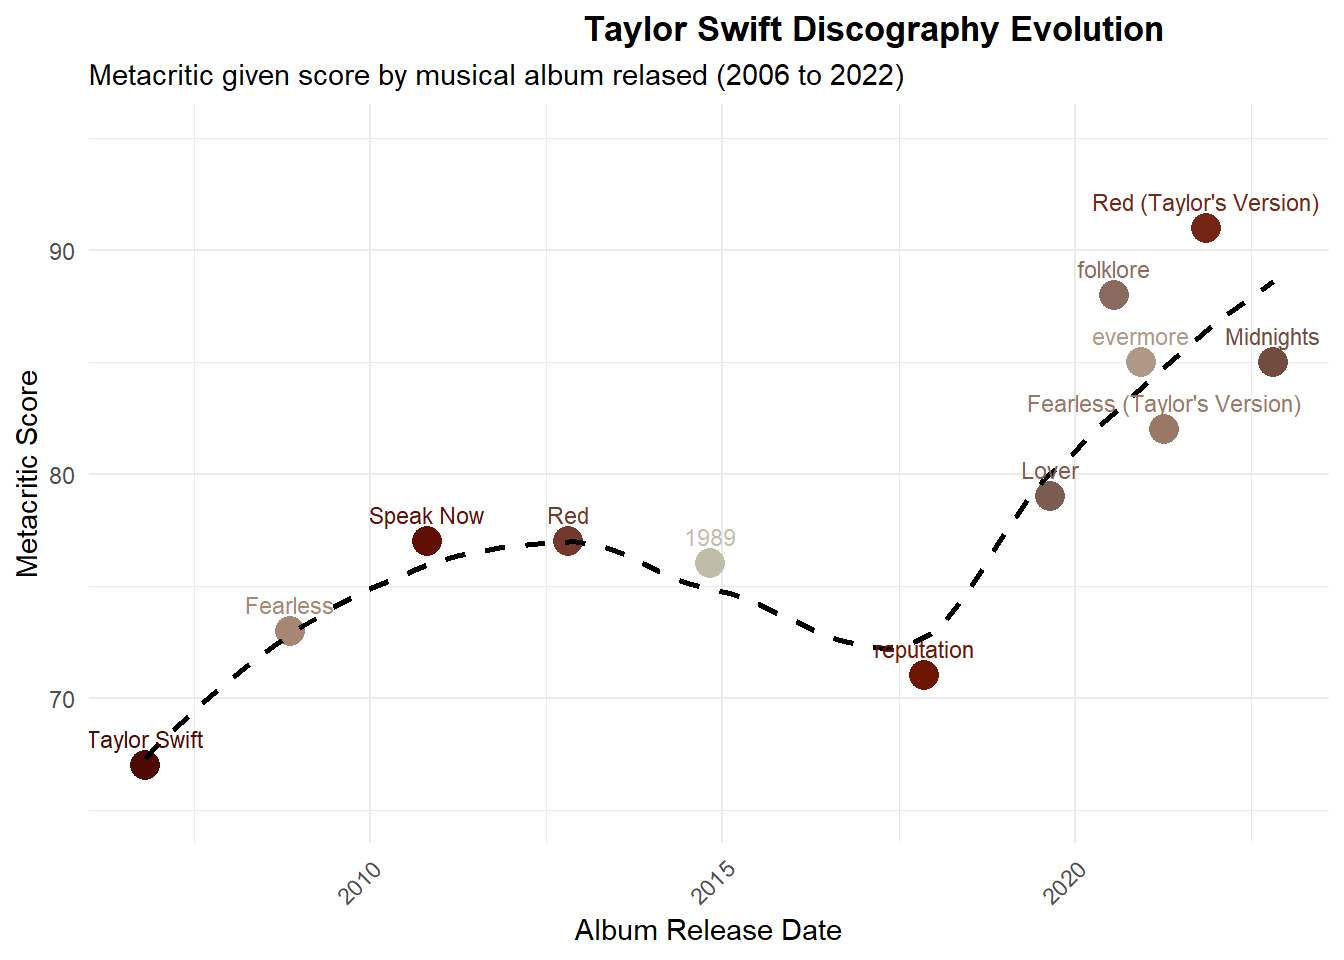
\includegraphics{Week07_hm_files/figure-latex/unnamed-chunk-3-1.pdf}

\#Make a Europe focused map 2020

\begin{Shaded}
\begin{Highlighting}[]
\CommentTok{\# Filter for the year 2020}
\NormalTok{plastics\_2020 }\OtherTok{\textless{}{-}}\NormalTok{ plastics }\SpecialCharTok{\%\textgreater{}\%}
  \FunctionTok{filter}\NormalTok{(year }\SpecialCharTok{==} \DecValTok{2020}\NormalTok{)}

\CommentTok{\# Summarize total plastic pollution by country for 2020}
\NormalTok{country\_summary }\OtherTok{\textless{}{-}}\NormalTok{ plastics\_2020 }\SpecialCharTok{\%\textgreater{}\%}
  \FunctionTok{group\_by}\NormalTok{(country) }\SpecialCharTok{\%\textgreater{}\%}
  \FunctionTok{summarize}\NormalTok{(}\AttributeTok{total\_plastic =} \FunctionTok{sum}\NormalTok{(grand\_total, }\AttributeTok{na.rm =} \ConstantTok{TRUE}\NormalTok{), }\AttributeTok{.groups =} \StringTok{\textquotesingle{}drop\textquotesingle{}}\NormalTok{)}

\CommentTok{\# Load world map data}
\NormalTok{world\_map }\OtherTok{\textless{}{-}} \FunctionTok{map\_data}\NormalTok{(}\StringTok{"world"}\NormalTok{)}

\CommentTok{\# Keep all European countries in the map, including those without data}
\NormalTok{europe\_map }\OtherTok{\textless{}{-}}\NormalTok{ world\_map }\SpecialCharTok{\%\textgreater{}\%}
  \FunctionTok{filter}\NormalTok{(region }\SpecialCharTok{\%in\%} \FunctionTok{unique}\NormalTok{(}\FunctionTok{c}\NormalTok{(country\_summary}\SpecialCharTok{$}\NormalTok{country, world\_map}\SpecialCharTok{$}\NormalTok{region)))}

\CommentTok{\# Merge the country summary with the world map data}
\NormalTok{map\_data }\OtherTok{\textless{}{-}}\NormalTok{ europe\_map }\SpecialCharTok{\%\textgreater{}\%}
  \FunctionTok{left\_join}\NormalTok{(country\_summary, }\AttributeTok{by =} \FunctionTok{c}\NormalTok{(}\StringTok{"region"} \OtherTok{=} \StringTok{"country"}\NormalTok{))}

\CommentTok{\# Plot the Europe map with zoom for 2020 data}
\FunctionTok{ggplot}\NormalTok{(}\AttributeTok{data =}\NormalTok{ map\_data) }\SpecialCharTok{+}
  \FunctionTok{geom\_polygon}\NormalTok{(}\FunctionTok{aes}\NormalTok{(}\AttributeTok{x =}\NormalTok{ long, }\AttributeTok{y =}\NormalTok{ lat, }\AttributeTok{group =}\NormalTok{ group, }\AttributeTok{fill =}\NormalTok{ total\_plastic), }\AttributeTok{color =} \StringTok{"black"}\NormalTok{) }\SpecialCharTok{+}
  \FunctionTok{scale\_fill\_viridis\_c}\NormalTok{(}\AttributeTok{na.value =} \StringTok{"gray"}\NormalTok{, }\AttributeTok{name =} \StringTok{"Total Plastic (units)"}\NormalTok{) }\SpecialCharTok{+}
  \FunctionTok{labs}\NormalTok{(}\AttributeTok{title =} \StringTok{"Plastic Pollution by Country in Europe (2020)"}\NormalTok{) }\SpecialCharTok{+}
  \FunctionTok{theme\_minimal}\NormalTok{() }\SpecialCharTok{+}
    \FunctionTok{theme}\NormalTok{(}\AttributeTok{plot.title =} \FunctionTok{element\_text}\NormalTok{(}\AttributeTok{hjust =} \FloatTok{0.5}\NormalTok{, }\AttributeTok{size =} \DecValTok{16}\NormalTok{, }\AttributeTok{face =} \StringTok{"bold"}\NormalTok{)) }\SpecialCharTok{+}  \CommentTok{\# Center title}
  \FunctionTok{coord\_fixed}\NormalTok{(}\AttributeTok{xlim =} \FunctionTok{c}\NormalTok{(}\SpecialCharTok{{-}}\DecValTok{10}\NormalTok{, }\DecValTok{40}\NormalTok{), }\AttributeTok{ylim =} \FunctionTok{c}\NormalTok{(}\DecValTok{35}\NormalTok{, }\DecValTok{60}\NormalTok{)) }\SpecialCharTok{+} \CommentTok{\#Adjust limits for zoom}
  \FunctionTok{annotation\_scale}\NormalTok{(}\AttributeTok{bar\_cols =} \FunctionTok{c}\NormalTok{(}\StringTok{"black"}\NormalTok{, }\StringTok{"white"}\NormalTok{), }\AttributeTok{location =} \StringTok{"bl"}\NormalTok{, }\AttributeTok{units =} \StringTok{"mi"}\NormalTok{ ) }\SpecialCharTok{+}
  \FunctionTok{annotation\_north\_arrow}\NormalTok{(}\AttributeTok{location =} \StringTok{"tr"}\NormalTok{,}
                       \AttributeTok{style =} \FunctionTok{north\_arrow\_fancy\_orienteering}\NormalTok{(),}
                       \AttributeTok{height =} \FunctionTok{unit}\NormalTok{(}\DecValTok{1}\NormalTok{, }\StringTok{"cm"}\NormalTok{),}
                       \AttributeTok{width =} \FunctionTok{unit}\NormalTok{(}\DecValTok{1}\NormalTok{, }\StringTok{"cm"}\NormalTok{),}
                       \AttributeTok{rotation =} \DecValTok{0}\NormalTok{)  }
\end{Highlighting}
\end{Shaded}

\includegraphics{Week07_hm_files/figure-latex/unnamed-chunk-4-1.pdf}

\end{document}
